\documentclass{beamer}
\usepackage[utf8]{inputenc}
\usepackage{tikz}
\usetikzlibrary{shapes.geometric, arrows}
\tikzstyle{std} = [rectangle, minimum width=2.5cm, minimum height=0.8cm, text centered, draw=black, fill=gray!30] 
\tikzstyle{arrow} = [double,->,>=stealth]
\addtobeamertemplate{navigation symbols}{}{%
    \usebeamerfont{footline}%
    \usebeamercolor[fg]{footline}%
    \hspace{1em}%
    \insertframenumber/\inserttotalframenumber
  }

%Information to be included in the title page:
\title{Spatial Price Competition: A Semiparametric Approach}
\author{Caio Figueiredo}
\institute{Penn State}
\date{2019}
 
\begin{document}
 
\frame{\titlepage}
 
\begin{frame}
  \frametitle{Introduction}
  \begin{itemize}
    \item Objective: develop an empirical technique that can be used to discriminate between local and global competition
    \item Immediate Application: Wholesale Gasoline Market
  \end{itemize}

\end{frame}

\begin{frame}
  \frametitle{Definitions}

  \begin{itemize}
    \item Local competition denotes a situation in which firms compete directly only with a subset of \textbf{closest} firms.
    \item In contrast, global competition denotes the scenario where a firm price is directly correlated to everyone else's price.
    \item Note that the notion of \textbf{closeness} is not yet defined and, in fact, it's definition is not always straightforward.
  \end{itemize}
\end{frame}

\begin{frame}
  \frametitle{Relevance}
  
  \begin{itemize}
    \item Competition characteristics such as  local/global are an important factor for defining a good policy.
  \end{itemize}

\end{frame}

\begin{frame}
  \frametitle{The Market}
    
  \center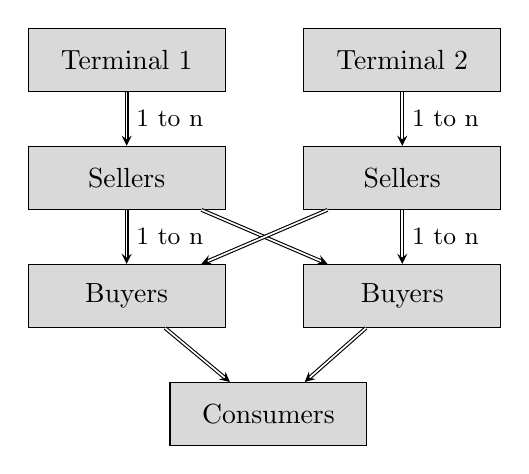
\begin{tikzpicture}[baseline=0, node distance=1.5cm]
    \node (term1) [std] {Terminal 1};
    \node (sel1)  [std, below of=term1] {Sellers};
    \node (buy1)  [std, below of=sel1] {Buyers};
    \node (end)  [std, below of=buy1, xshift=1.8cm] {Consumers};

    \node (term2) [std, right of=term1, xshift=2cm] {Terminal 2};
    \node (sel2)  [std, below of=term2] {Sellers};
    \node (buy2)  [std, below of=sel2] {Buyers};

    \draw [arrow] (term1) -- (sel1) node[midway, right] {\small{1 to n}};
    \draw [arrow] (sel1) -- (buy1) node[midway, right] {\small{1 to n}};
    \draw [arrow] (buy1) -- (end);

    \draw [arrow] (term2) -- (sel2) node[midway, right] {\small{1 to n}};
    \draw [arrow] (sel2) -- (buy2) node[midway, right] {\small{1 to n}};
    \draw [arrow] (buy2) -- (end);

    \draw [arrow] (sel1) -- (buy2);
    \draw [arrow] (sel2) -- (buy1);

  \end{tikzpicture}
\end{frame}

\begin{frame}
  \frametitle{The Market}
  \begin{itemize}
    \item Gasoline is piped by multiple sellers to terminal locations.
    \item Upstream Market: Sellers offer branded gas to long term binded buyers and unbranded gas to independent buyers
    \item Downstream Market: Buyers offer gasoline to consumers.
      \begin{itemize}
        \item[-] \small{We assume that the Downstream market is competitive, therefore the Downstream market price (SPOT price) is taken as given.}
      \end{itemize}
  \end{itemize}
\end{frame}

\begin{frame}
  \frametitle{The Market}
  \begin{itemize}
    \item We are interest in the inter-terminal unbranded gasoline market
      \begin{itemize}
        \item \textbf{We want to show that this market is locally competitive}
      \end{itemize}
    \item Since branded gasoline buyers are binded to sellers there is no inter-terminal branded market
  \end{itemize}
\end{frame}

\begin{frame}
  \frametitle{The model}
  \begin{itemize}
    \item We have $n$ Sellers:
      \begin{itemize}
        \item[-] $q = (q_1, q_2, ..., q_n)$ denotes the quantity sold.
        \item[-] $y = (y_1, y_2, ..., y_n)$ denotes product characteristics.
        \item[-] $\tilde{p}= (\tilde{p}_1, \tilde{p}_2, ..., \tilde{p}_n)$ denotes sellers price.
      \end{itemize}
    \item and $K$ Buyers:
      \begin{itemize}
        \item[-] $\tilde{v} = (\tilde{v}_1, \tilde{v_2}, ..., \tilde{v}_n)$ denotes buyers reselling price.
        \item[-] $\tilde{\Pi}(\tilde{v}, \tilde{p}, \tilde{y}) = \tilde{\pi}_k(v_k, \tilde{p}, \tilde{y})$ denotes buyers profit function.
      \end{itemize}
  \end{itemize}
\end{frame}

\begin{frame}
  \frametitle{The model}
  \begin{itemize}
    \item By defining:
      \begin{itemize}
        \item[-] $V$ a price index.
        \item[-] $p = V^{-1}\tilde{p}$.
        \item[-] $\bar{v} = V^{-1}\tilde{v}$.
      \end{itemize}
    \item We can approximate the profit function by:
  \end{itemize}
  \vspace{2mm}
  \footnotesize\[ \tilde{\Pi}(\tilde{v}, \tilde{p}, y) \approx V \left\{ \tilde{\alpha}^T_1p + \tilde{\alpha}_2 + \frac{V}{2}\left[p^TB^1p + \bar{v}B^2\bar{v} + p^TB^3\bar{v}\right] + \frac{1}{2}\left[p^TB^4y + \bar{v}B^5y\right]\right\}.  \]

  \begin{itemize}
    \item But since $\bar{v}$ is constant, because the downstream market is competitive, we can rewrite the above as:
  \end{itemize}

  \footnotesize\[ \Pi(p, y) = a_0 + a^Tp + \bar{a}^Ty + \frac{1}{2}\left[p^TB^1p + p^TB^4y\right] \]

\end{frame}

\begin{frame}
  \frametitle{The model}
  \begin{itemize}
    \item We can use Hotelling's Lemma to derive the demand function as:
  \end{itemize}

  \[ q_i = \frac{\partial \tilde{\Pi}}{\partial \tilde{p_i}} \approx \frac{\partial\Pi}{\partial p_i}\frac{\partial p_i}{\partial \tilde{p_i}} = \partial \frac{\Pi}{p_i} = a_i + \sum_{j=1} [b^1_{ij}p_j + b^4_{ij}y_j] \]

  \begin{itemize}
    \item Given the demand function we can derive the maximization problem of the upstream firms:
  \end{itemize}

  \[ \max_{p_i} (p_i - \gamma^Tc_i)\left[a_i + \sum_{j=1} [b^1_{ij}p_j + b^4_{ij}y_j] \right] - F_i \]

  \begin{itemize}
    \item Where $\gamma^Tc_i$ is the total variable cost and $F_i$ is the fixed cost.
  \end{itemize}
  
\end{frame}

\begin{frame}
  \frametitle{The model}
  \begin{itemize}
    \item Solving the sellers maximization problem we have:
  \end{itemize}

  \[ p_i = \frac{1}{-2b^1_{ii}}\left(a_i - b^1_{ii}\gamma^Tc_i + \sum_{j\ne i} b^1_{ij}p_j + \sum_{j=1} b^4_{ij}y_j \right)\ \forall i \in {1, ..., n} \]

\end{frame}

\begin{frame}
  \frametitle{The model}
  \begin{itemize}
    \item Now we can aggregate costs factors and product characteristics to have the follow econometrical model:
  \end{itemize}

  \[ p  = A + X\beta + Gp + u \]

  \begin{itemize}
    \item Where:
      \begin{itemize}
        \item[-] $A$ is a vector of intercepts that is treated as random effects.
        \item[-] $X$ is a matrix of control variables
        \item[-] $\beta$ is a vector of parameters.
        \item[-] $G = (g_{ij}$) is a matrix such that: $g_{ii} = 0\ \forall i$ and $g_{ij} = g(d_{ij})\ \forall i \ne j$.
      \end{itemize}
    \item \textbf{$g$ will be estimated using a Semiparametric approach}
  \end{itemize}
\end{frame}

\begin{frame}
  \frametitle{Conventional Method}
  \begin{itemize}
    \item If one is willing to impose considerable structure previous equation, it is possible to estimate it by conventional methods.
    \item Particularly, if we assume that $u_i \sim $i.i.d.$N(0, \sigma^2)$ and that $G = \psi\mathcal{W}$, where $\psi$ is a parameter (it's a scalar) and $\mathcal{W}$ is a weighting matrix (of distances), then the parameters ($\sigma^2, \beta, \psi$) can be estimated by standard OLS.

  %\footnotesize\[ - \frac{N}{2} \ln(2\pi\sigma^2) + \ln |I_n - \psi \mathcal{W}| - \frac{1}{2\sigma^2}(p - \psi \mathcal{W}p - X \beta)^T(p - \psi\mathcal{W}p - X\beta) \]

  \item Which is a common approach in the literature
  \end{itemize}
  
\end{frame}

\begin{frame}
  \frametitle{Semiparametric method}
  \begin{itemize}
    \item $g(d)$ can be written as:
      \[g(d) = \sum^{\infty}_{l=1} \alpha_l e_l(d)\]
    \item where $e_l(d)$ is the basis of the functional space (we usually have: $e_l = d^l$)
    \item and therefore:
      \[p_i  = a_i + \sum^{\infty}_{l=1} \alpha_l \sum_{j\ne i} e_l(d_{ij})p_j + \beta^Tx_i + u_i \]
  \end{itemize}
\end{frame}

\begin{frame}
  \frametitle{Semiparametric method}

  \begin{itemize}
    \item By truncating the number of expansions terms to be estimated, we have:
      \[p_i  = a_i + sum^{L_n}_{l=1} \alpha_l \sum_{j\ne i} e_l(d_{ij})p_j + \beta^Tx_i + v_i \]
    \item Where $v_i = u_i + \sum^{\infty}_{l=L_n+1} \alpha_l \sum_{j\ne i} e_l(d_{ij})p_j$
    \item Rewriting in vector notation:
      \[p = Z \alpha + X \beta  + v\]
    \item Where $Z$ is a whose $(l,i)$ element is $\sum_{j\ne i} e_l(d_{ij})p_j$.
    \item \textbf{Which can be estimated by OLS}.
  \end{itemize}
  
\end{frame}

\begin{frame}
  \frametitle{Application visualization}

  \begin{itemize}
    \item In the Wholesale Gasoline Market application, $L_n$ is set to $5$, using $e_l(d) = d^l$, we have:
      \[p_i  =  a_i + \sum_{j\ne i} (\alpha_1d_{ij} + \alpha_2d^2_{ij} + \alpha_3d^3_{ij} + \alpha_4d^4_{ij} + \alpha_5d^5_{ij})p_j + \beta^Tx_i + v_i \]
  \end{itemize}
  
\end{frame}

\begin{frame}
  \frametitle{Problem}
  \begin{itemize}
    \item Rival price ($p_j$) is not independent of $u_i$, let alone $v_i$
    \item \textbf{This endogeneity problem is dealt by the use of Instrumental Variables}
    \item If $H$ is the size o $X$, we must have at least $H + L_n$ instruments.
  \end{itemize}
\end{frame}

\begin{frame}
  \frametitle{Estimator}

  \begin{itemize}
    \item By defining $W$ as the concatenation of $X$ and $Z$ and $\theta = [\alpha^T. \beta^T]^T$, we are able to use a standard IV estimator:
      \[ \hat{\theta} = (W^TP_BW)^-1W^TP_Bp \]
    \item Where $P_B$ is the orthogonal projection matrix of the matrix of instruments.
    \item and hence:
      \[\hat{g}(d) = \sum^{L_n}_{l=1}\hat{\alpha}_le_l(d) \]
  \end{itemize}
  
\end{frame}

\begin{frame}
  \frametitle{Theorems}

  \begin{itemize}
    \item Theorem 1 (Consistency): $\hat{g}(d) - g(d) = o_p(1)$ for \textit{almost all} $d$ and $\hat{\beta} - \beta = o_p(1)$
    \item Theorem 2 (Asymptotic Normality of $\hat{\beta}$):
      \[(X^TP_BM_{P_BZ}P_B\Omega M_{P_BZ}P_BX)^{1/2}X^TP_BM_{P_BZ}P_BX(\hat{\beta} - \beta) \underrightarrow{\mathcal{L}} N(0,I)\]
    \item Theorem 3 (Asymptotic Normality of $\hat{g}$): 
      \[ \hat{\Omega}^{-1/2}_g\{\hat{g}(d) - g(d)\} \underrightarrow{\mathcal{L}} N(0,1) \]
    \item The theorems are proved in the papers but the proofs are going to be skipped in this presentation.
  \end{itemize}
\end{frame}

\begin{frame}
  \frametitle{Remmember our application}
    
  \center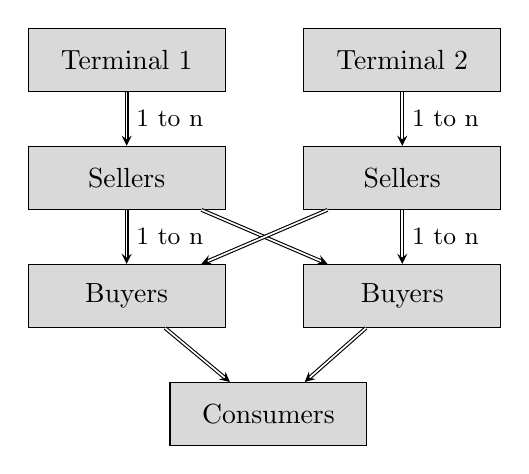
\begin{tikzpicture}[baseline=0, node distance=1.5cm]
    \node (term1) [std] {Terminal 1};
    \node (sel1)  [std, below of=term1] {Sellers};
    \node (buy1)  [std, below of=sel1] {Buyers};
    \node (end)  [std, below of=buy1, xshift=1.8cm] {Consumers};

    \node (term2) [std, right of=term1, xshift=2cm] {Terminal 2};
    \node (sel2)  [std, below of=term2] {Sellers};
    \node (buy2)  [std, below of=sel2] {Buyers};

    \draw [arrow] (term1) -- (sel1) node[midway, right] {\small{1 to n}};
    \draw [arrow] (sel1) -- (buy1) node[midway, right] {\small{1 to n}};
    \draw [arrow] (buy1) -- (end);

    \draw [arrow] (term2) -- (sel2) node[midway, right] {\small{1 to n}};
    \draw [arrow] (sel2) -- (buy2) node[midway, right] {\small{1 to n}};
    \draw [arrow] (buy2) -- (end);

    \draw [arrow] (sel1) -- (buy2);
    \draw [arrow] (sel2) -- (buy1);

  \end{tikzpicture}
\end{frame}

\begin{frame}
  \frametitle{Data}

  \begin{itemize}
    \item Our data is a cross section of 305 terminals in the lower 48 states.
    \item Our main variable of interest is the (lowest) unbranded gasoline price per terminal, which is collect by Oil Price Information Service (OPIS):

    \item \textit{PRICE} - regular unleaded price for the 3rd week in October of 1993
  \end{itemize}
\end{frame}

\begin{frame}
  \frametitle{Data, components of X:}
  \footnotesize\begin{itemize}
    \item \textit{SPOT} - gasoline spot prices to capture overall economic conditions in the oil industry
    \item \textit{STOCK} - the percentage change in stocks to measure of supply/demand imbalance
    \item \textit{POP} - city population for local demand variables
    \item \textit{INC} - city household income for local demand variables
    \item \textit{WAGE} - city wage rates to measure local labor costs
    \item \textit{MTBE} - indicator for regions that require that gasoline burned in the region contain methyl terciary butyl, which increases production costs
    \item \textit{NCOMP} - the number of competing sellers at a terminal to capture variations in local market structure
    \item \textit{BRPRICE} - average branded price for each terminal
    \item \textit{NBRAND} - the number of branded sellers at that terminal
    \item \textit{PAD} - dummy variables that distinguish the five petroleum allocation districts
  \end{itemize}
\end{frame}

\begin{frame}
  \frametitle{Data, distances measures:}
  \begin{itemize}
    \item[1.] \textbf{NNX} - dummy variables that equal one if outlet $j$ is $i$'s nearest neighbor and zero otherwise, where $i$'s nearest neighbor is located in the terminal that is the shortest Euclidean distance from $i$ \\
      \textbf{NNP} - the nearest neighbor determined endogenously by prices and transport costs. That is, Terminal B is the nearest neighbor of Terminal A, if B is chepeast alternative to A.
    \item[2.] \textbf{CBX} - dummy variables that equal one if $i$ and $j$ share an exogenous market boundary but are not nearest neighbors, and zero otherwise \\
      \textbf{CBP} - similar to \textit{CBX} except that market boundaries are endogenously determined
  \end{itemize}
\end{frame}


\begin{frame}
  \frametitle{CBP Illustration}
  \begin{figure}
    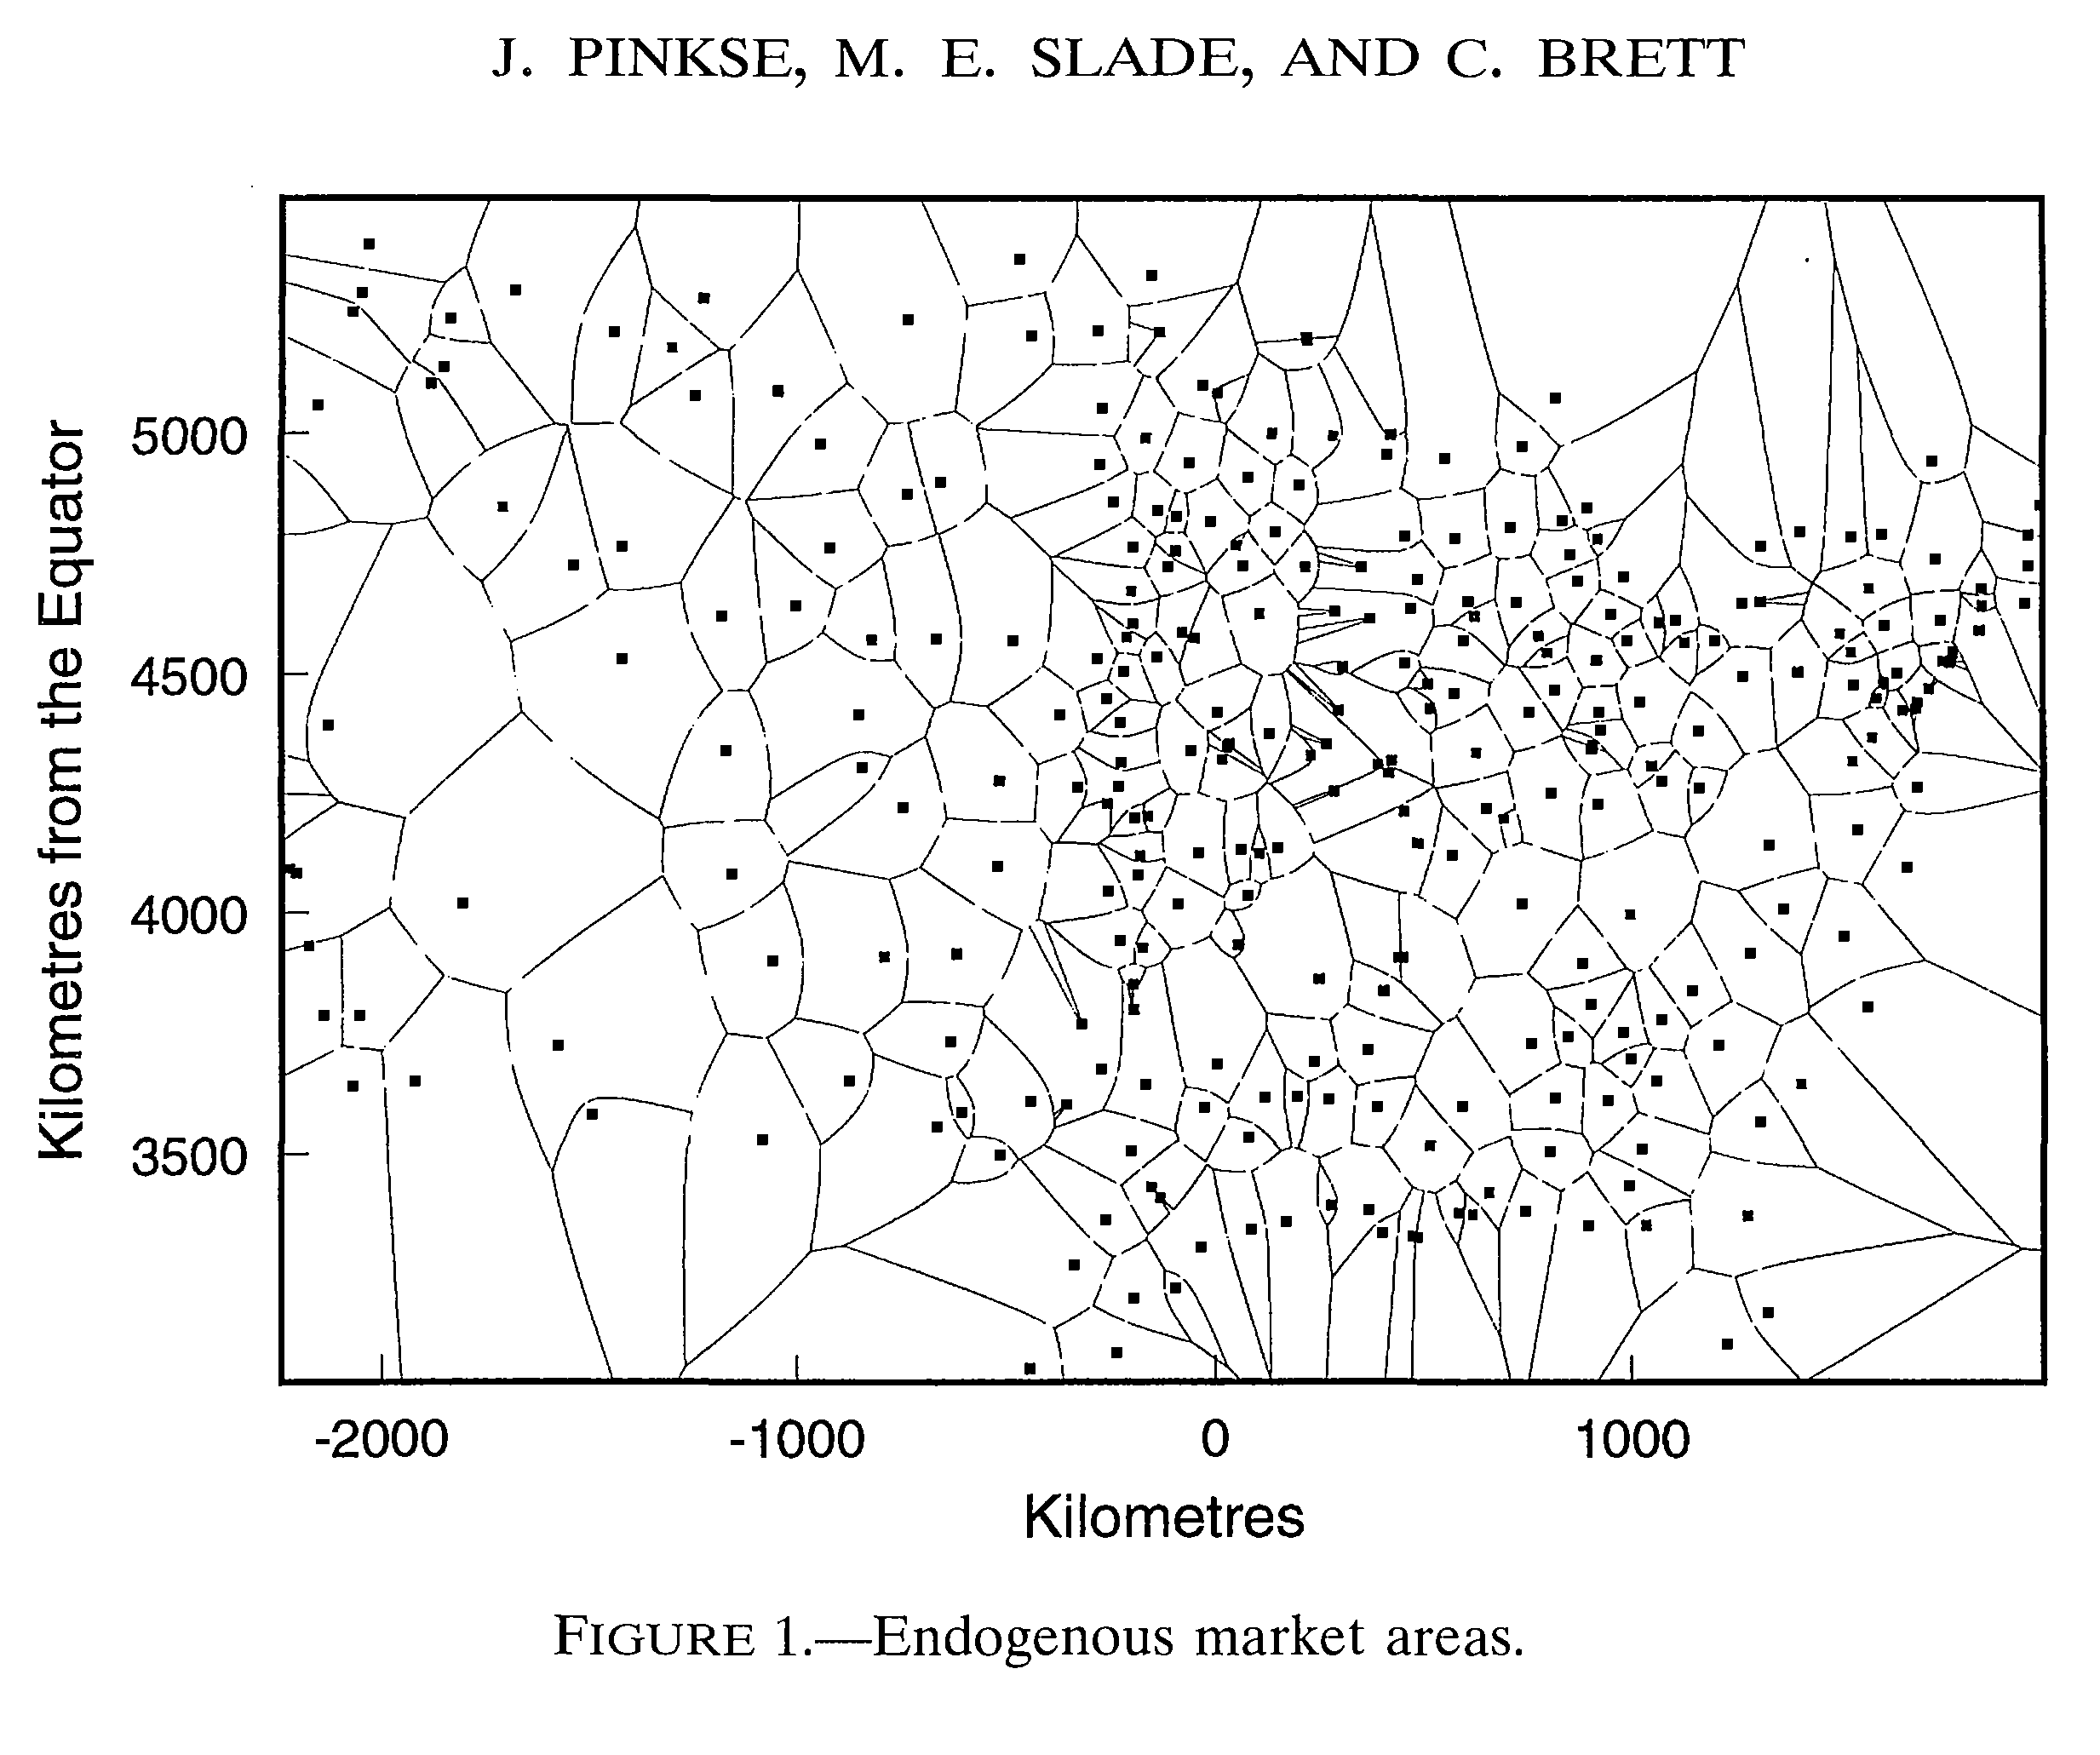
\includegraphics[width=\linewidth]{CBN.png}
  \end{figure}
\end{frame}

\begin{frame}
  \frametitle{Data, distances measures:}
  \begin{itemize}
    \item[3.] \textbf{CBX2} - dummy variables that equal one if $i$ and $j$ do not share a market boundary in the sense of \textit{CBX}, but each shares a boundary with a third seller \\
      \textbf{CBP2} - similar to \textit{CBX2} except that markets are based on delivery prices instead of Euclidean distances. 
    \item[4.] \textbf{EDX} - global measures of closeness, which is the function of the Euclidean distance between locations $i$ and $j$, $\frac{1}{(0.01 \times XX_{ij} + 1)}$ where $XX_{ij} = EU_{ij}$ \\
      \textbf{EDP} - similar to \textit{EDP} except that $XX_{ij} = EU_{ij} + \frac{(p_j - p_i)}{\tau}$, which means functions are of delivered prices
  \end{itemize}
\end{frame} 

\begin{frame}
  \frametitle{OLS results}
  \vspace{-0.5cm}
  \begin{figure}
    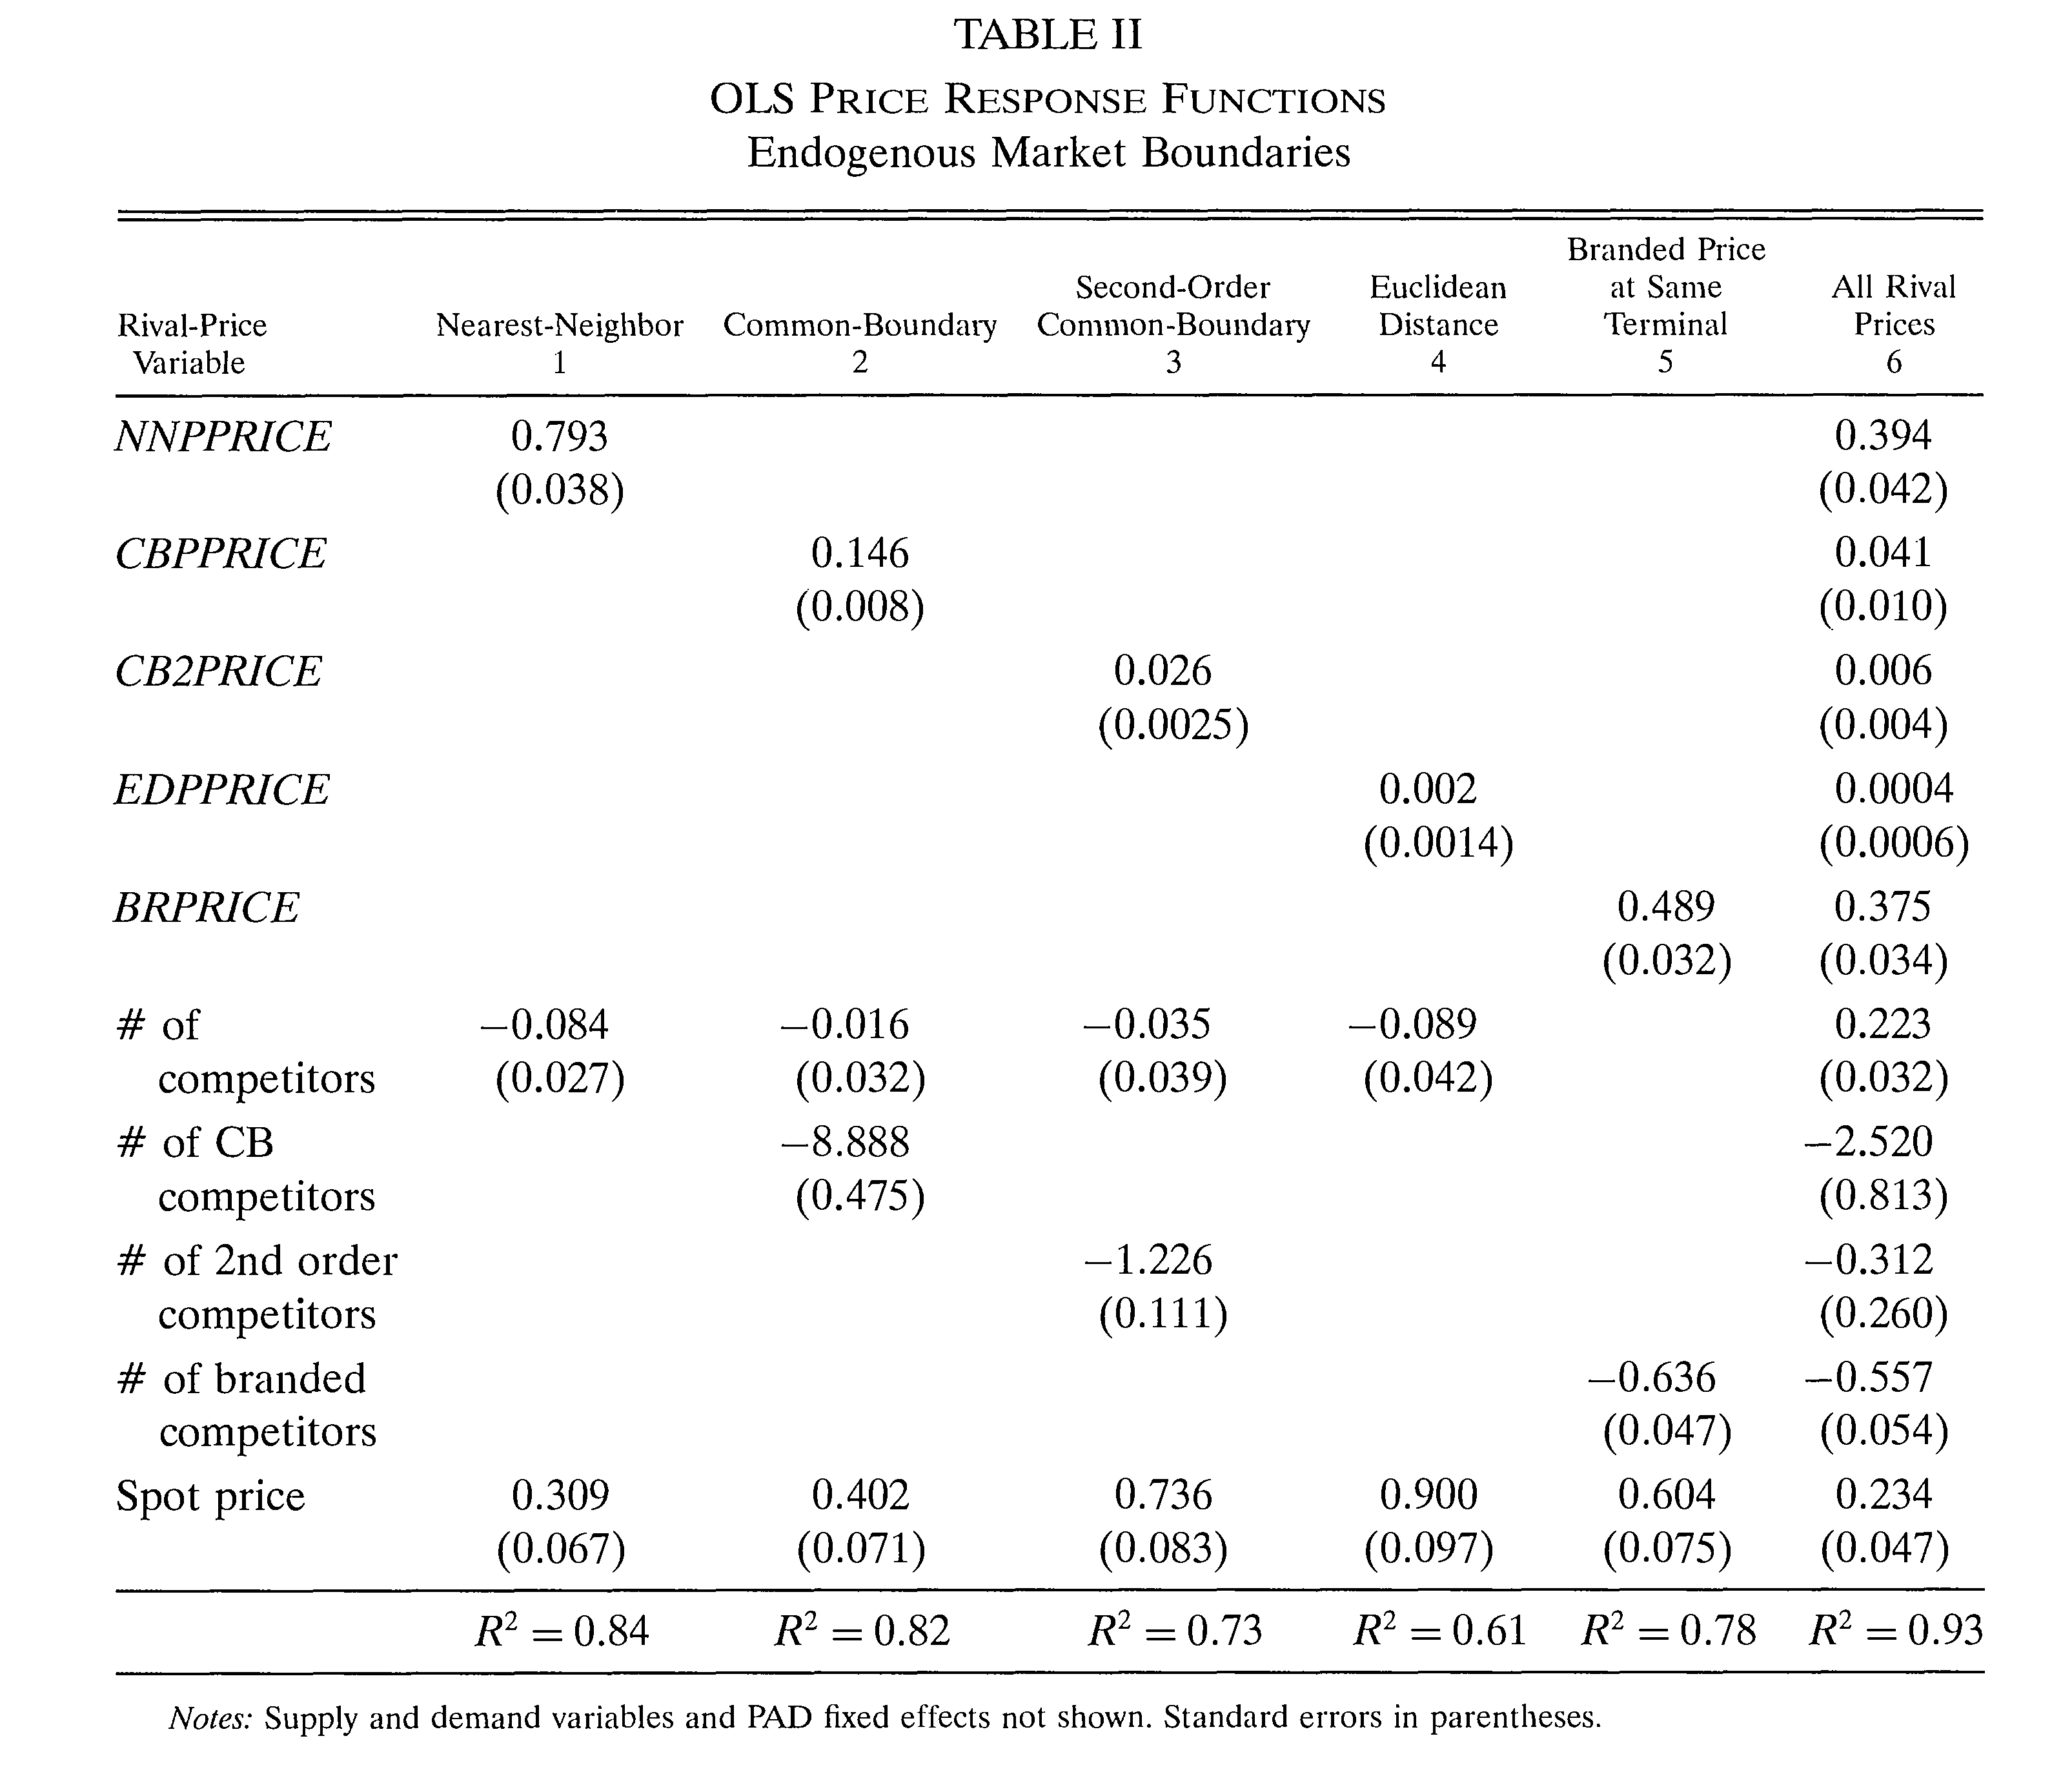
\includegraphics[width=\linewidth, height= 8cm]{OLS_res.png}
  \end{figure}
\end{frame}

\begin{frame}
  \frametitle{Data, the instruments:}
  \begin{itemize}
    \item \textbf{Both rival prices and distances can be endogenous.}
    \item We create instruments by multiplying terminal-specific exogenous variable (i.e. population, income, wage, etc..) by an exogeneous weighting matrix. To illustrate, when a specification includes the NNP, instruments are creating by multiplying NNP and POP, INC, etc...:
      \[p_i = a_i + \beta x_i + \alpha g(NNP) \times p_j + \lambda NNX \times X + u \]
  \end{itemize}
\end{frame}

\begin{frame}
  \frametitle{IV results}
  \vspace{-0.6cm}
  \begin{figure}
    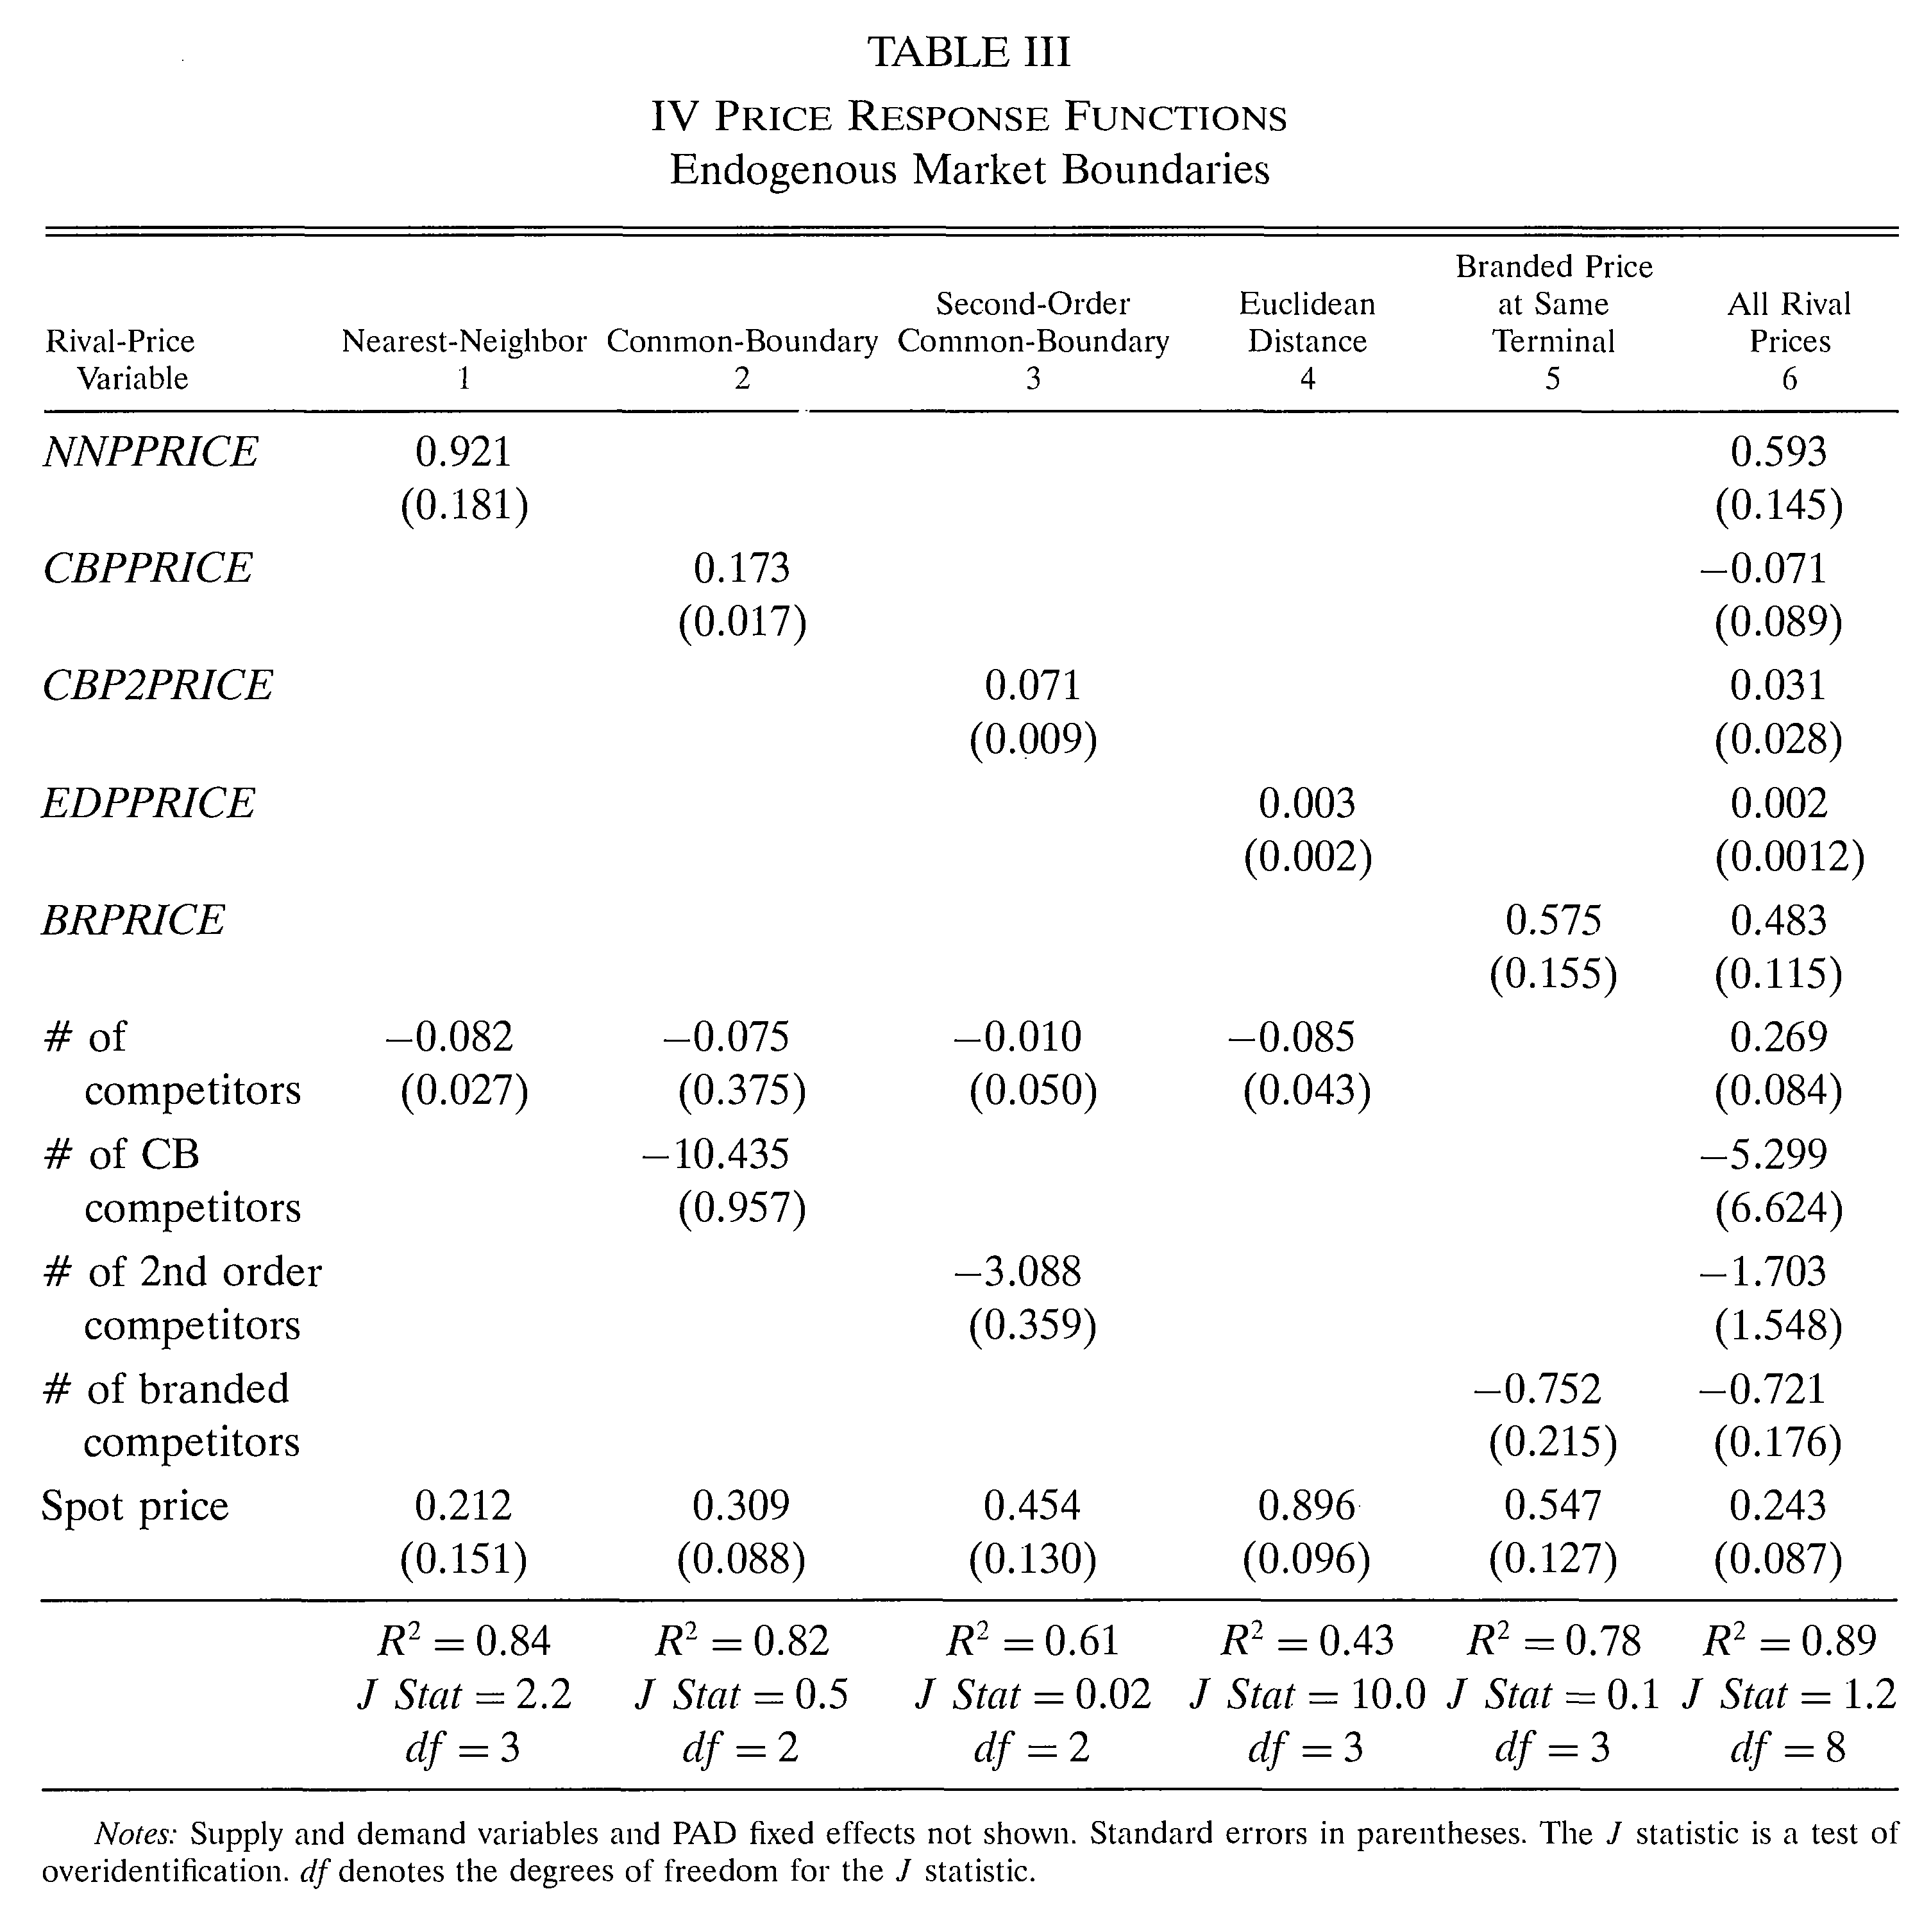
\includegraphics[width=\linewidth, height=9.3cm]{IV_res.png}
  \end{figure}
\end{frame}

\begin{frame}
  \frametitle{Finally, Semiparametric model}

  \begin{itemize}
    \item $g(d)$ is approximated by a 5-order expasions
    \item The increase in the number of parameters demand an increase in the number of instruments, which is achieved by creating by multiplying the exogenous variable by $e_l(d_{ij})$

  \end{itemize}
\end{frame}

\begin{frame}
  \frametitle{Semiparametric model}
  
  \begin{itemize}
    \item In all semiparametric model $g(d)$ is the result of a compound of the discrete measures NNP, CPB and CPB2 with the continuous measure EDX, such that:
      \[ g(d) = \sum_{t = \{0,1\}} \textbf{1}(d_D = t)g^t(d_C) \]
    \item We expect $g^0(d) = 0$.
    \item We are interest in $g^1(d)$.
  \end{itemize}
\end{frame}

\begin{frame}
  \frametitle{Semiparametric results}
  \vspace{-0.6cm}
  \begin{figure}
    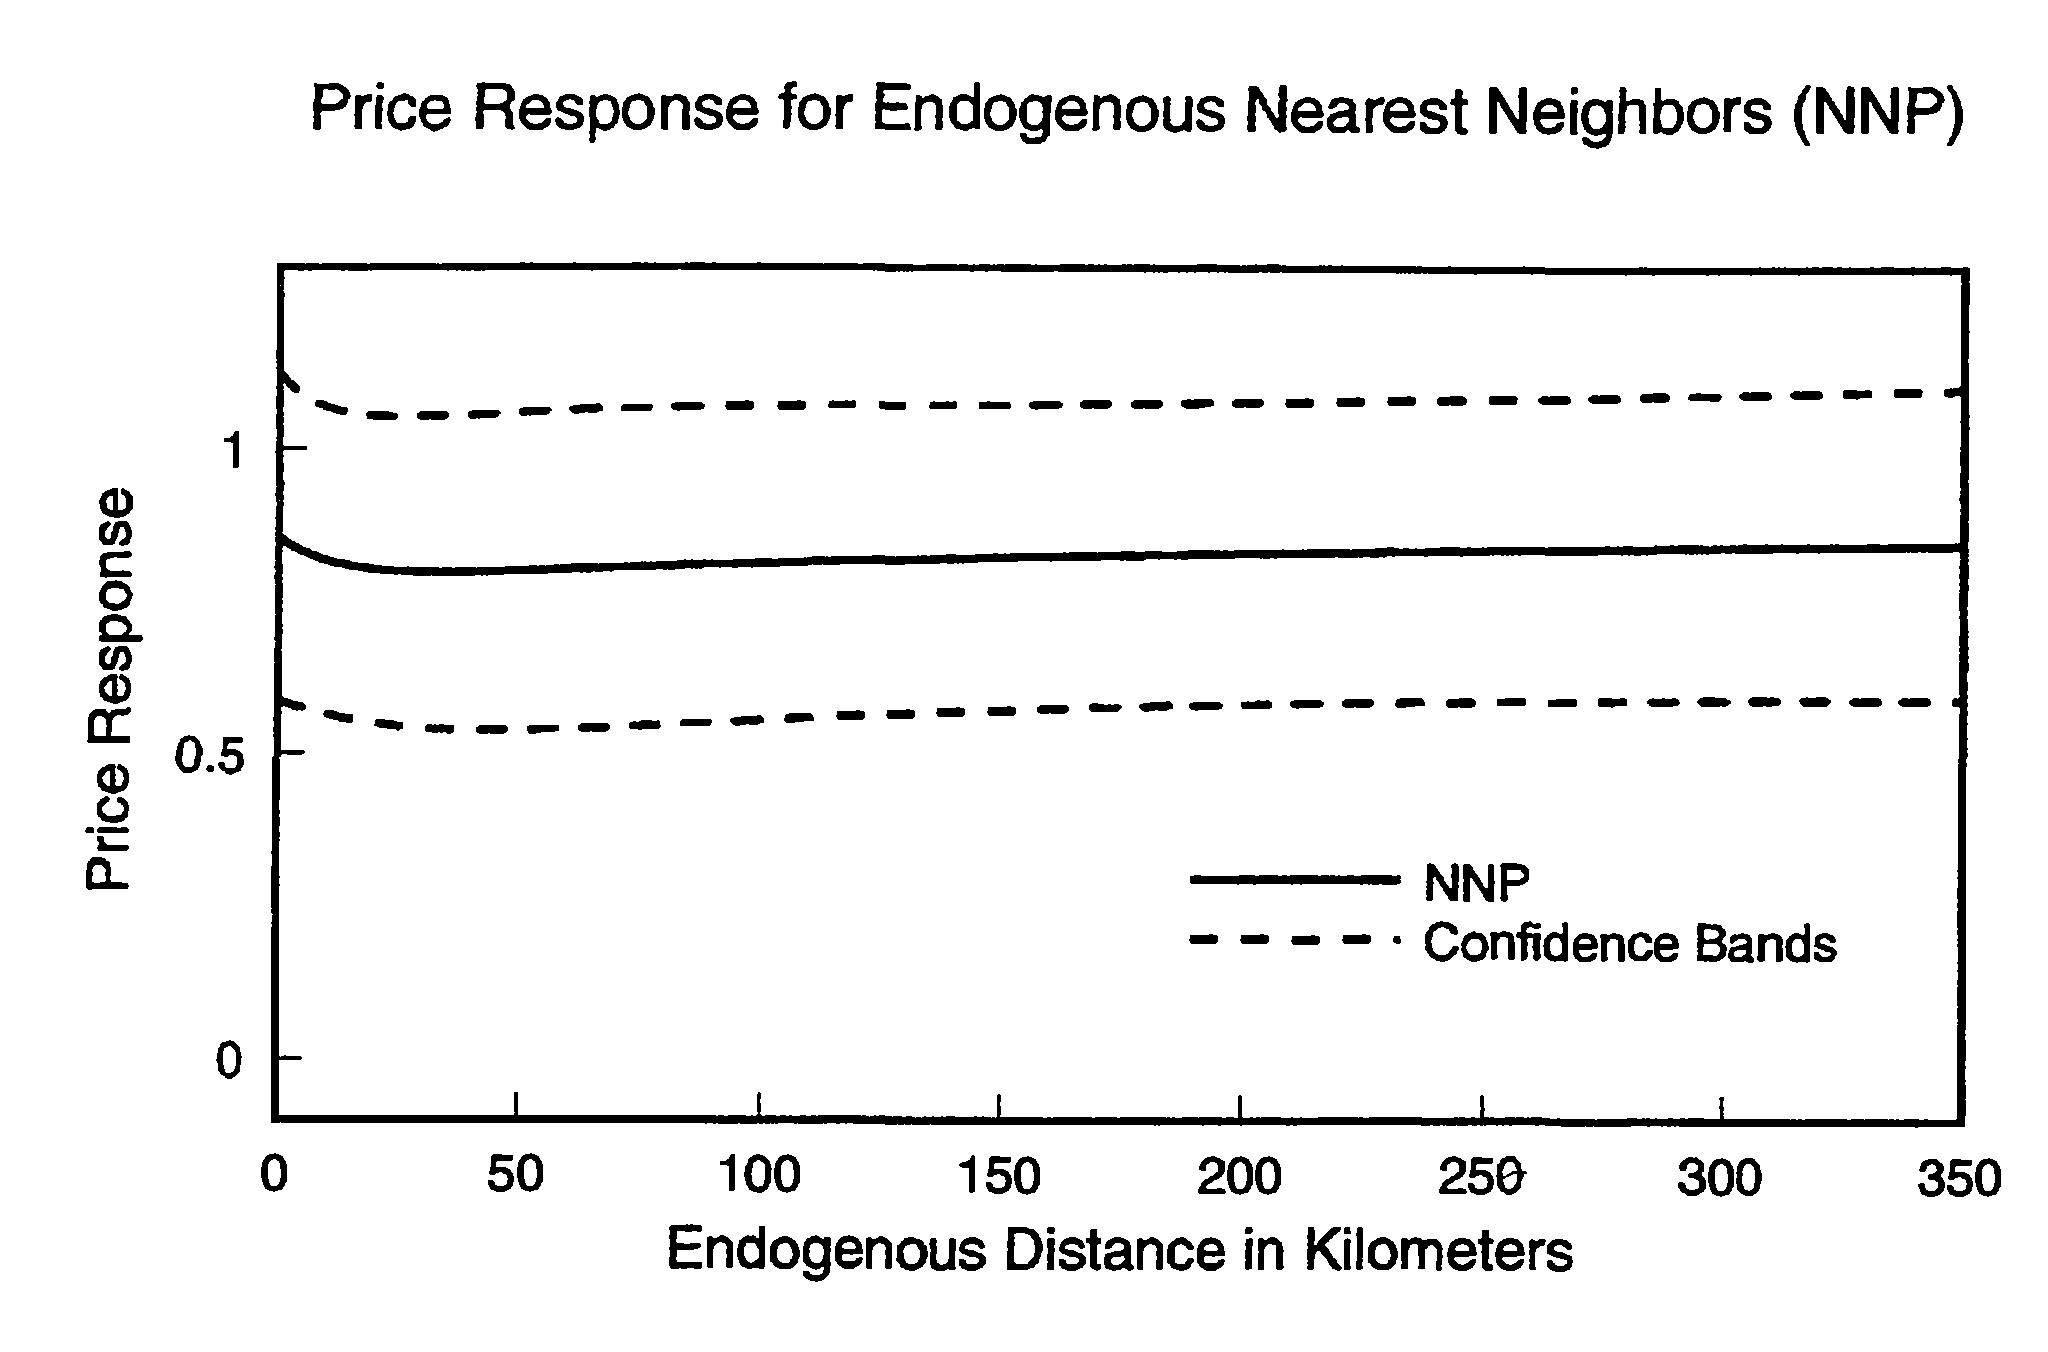
\includegraphics[width=\linewidth]{NNP.png}
  \end{figure}
\end{frame}

\begin{frame}
  \frametitle{Semiparametric results}
  \vspace{-0.6cm}
  \begin{figure}
    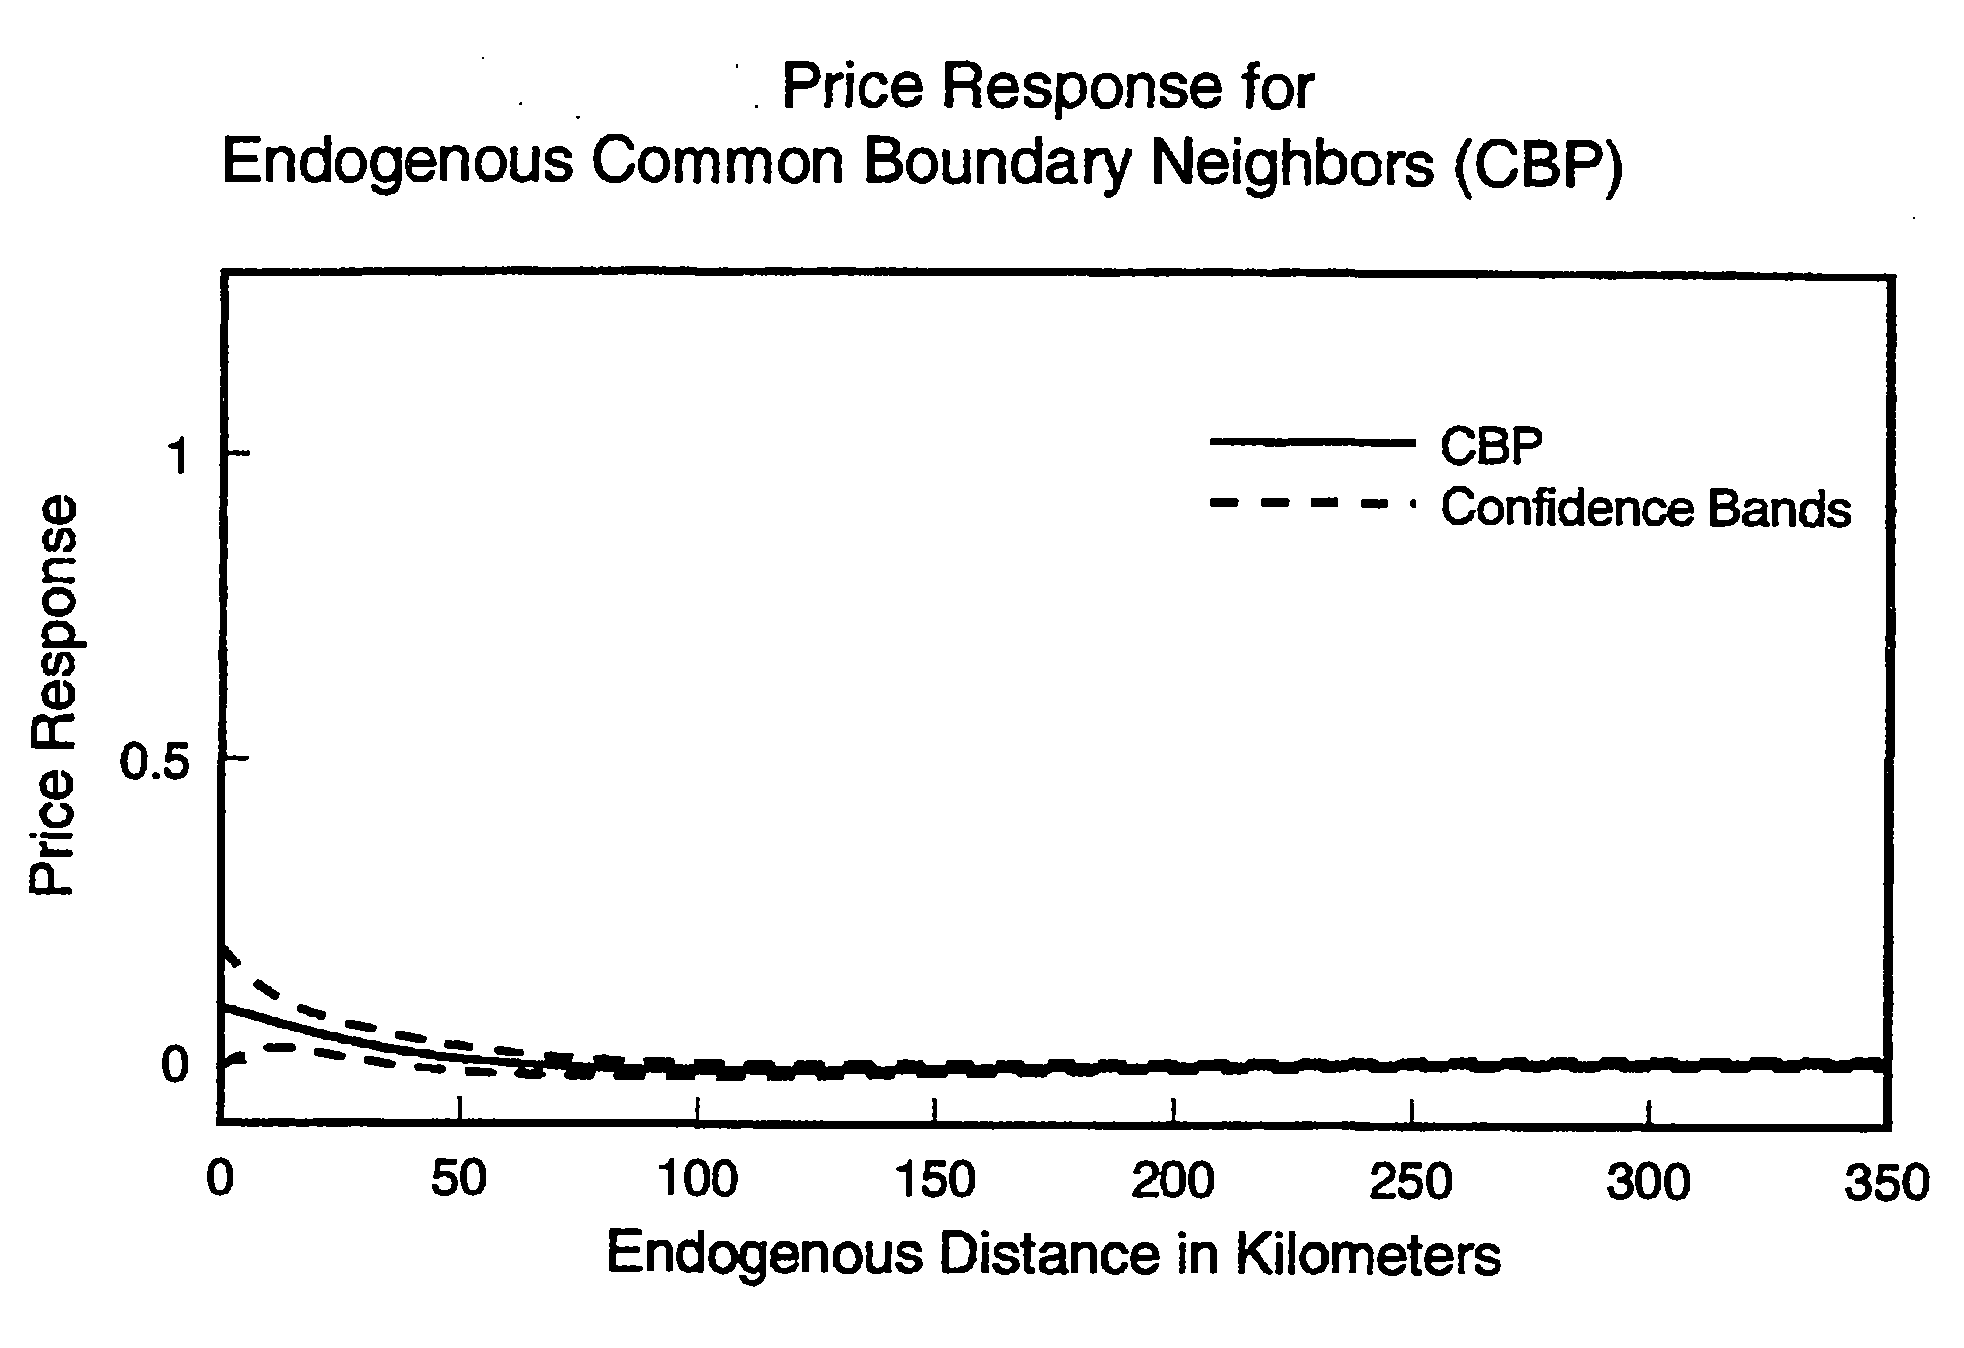
\includegraphics[width=\linewidth]{CBP.png}
  \end{figure}
\end{frame}

\begin{frame}
  \frametitle{Semiparametric results}
  \vspace{-0.6cm}
  \begin{figure}
    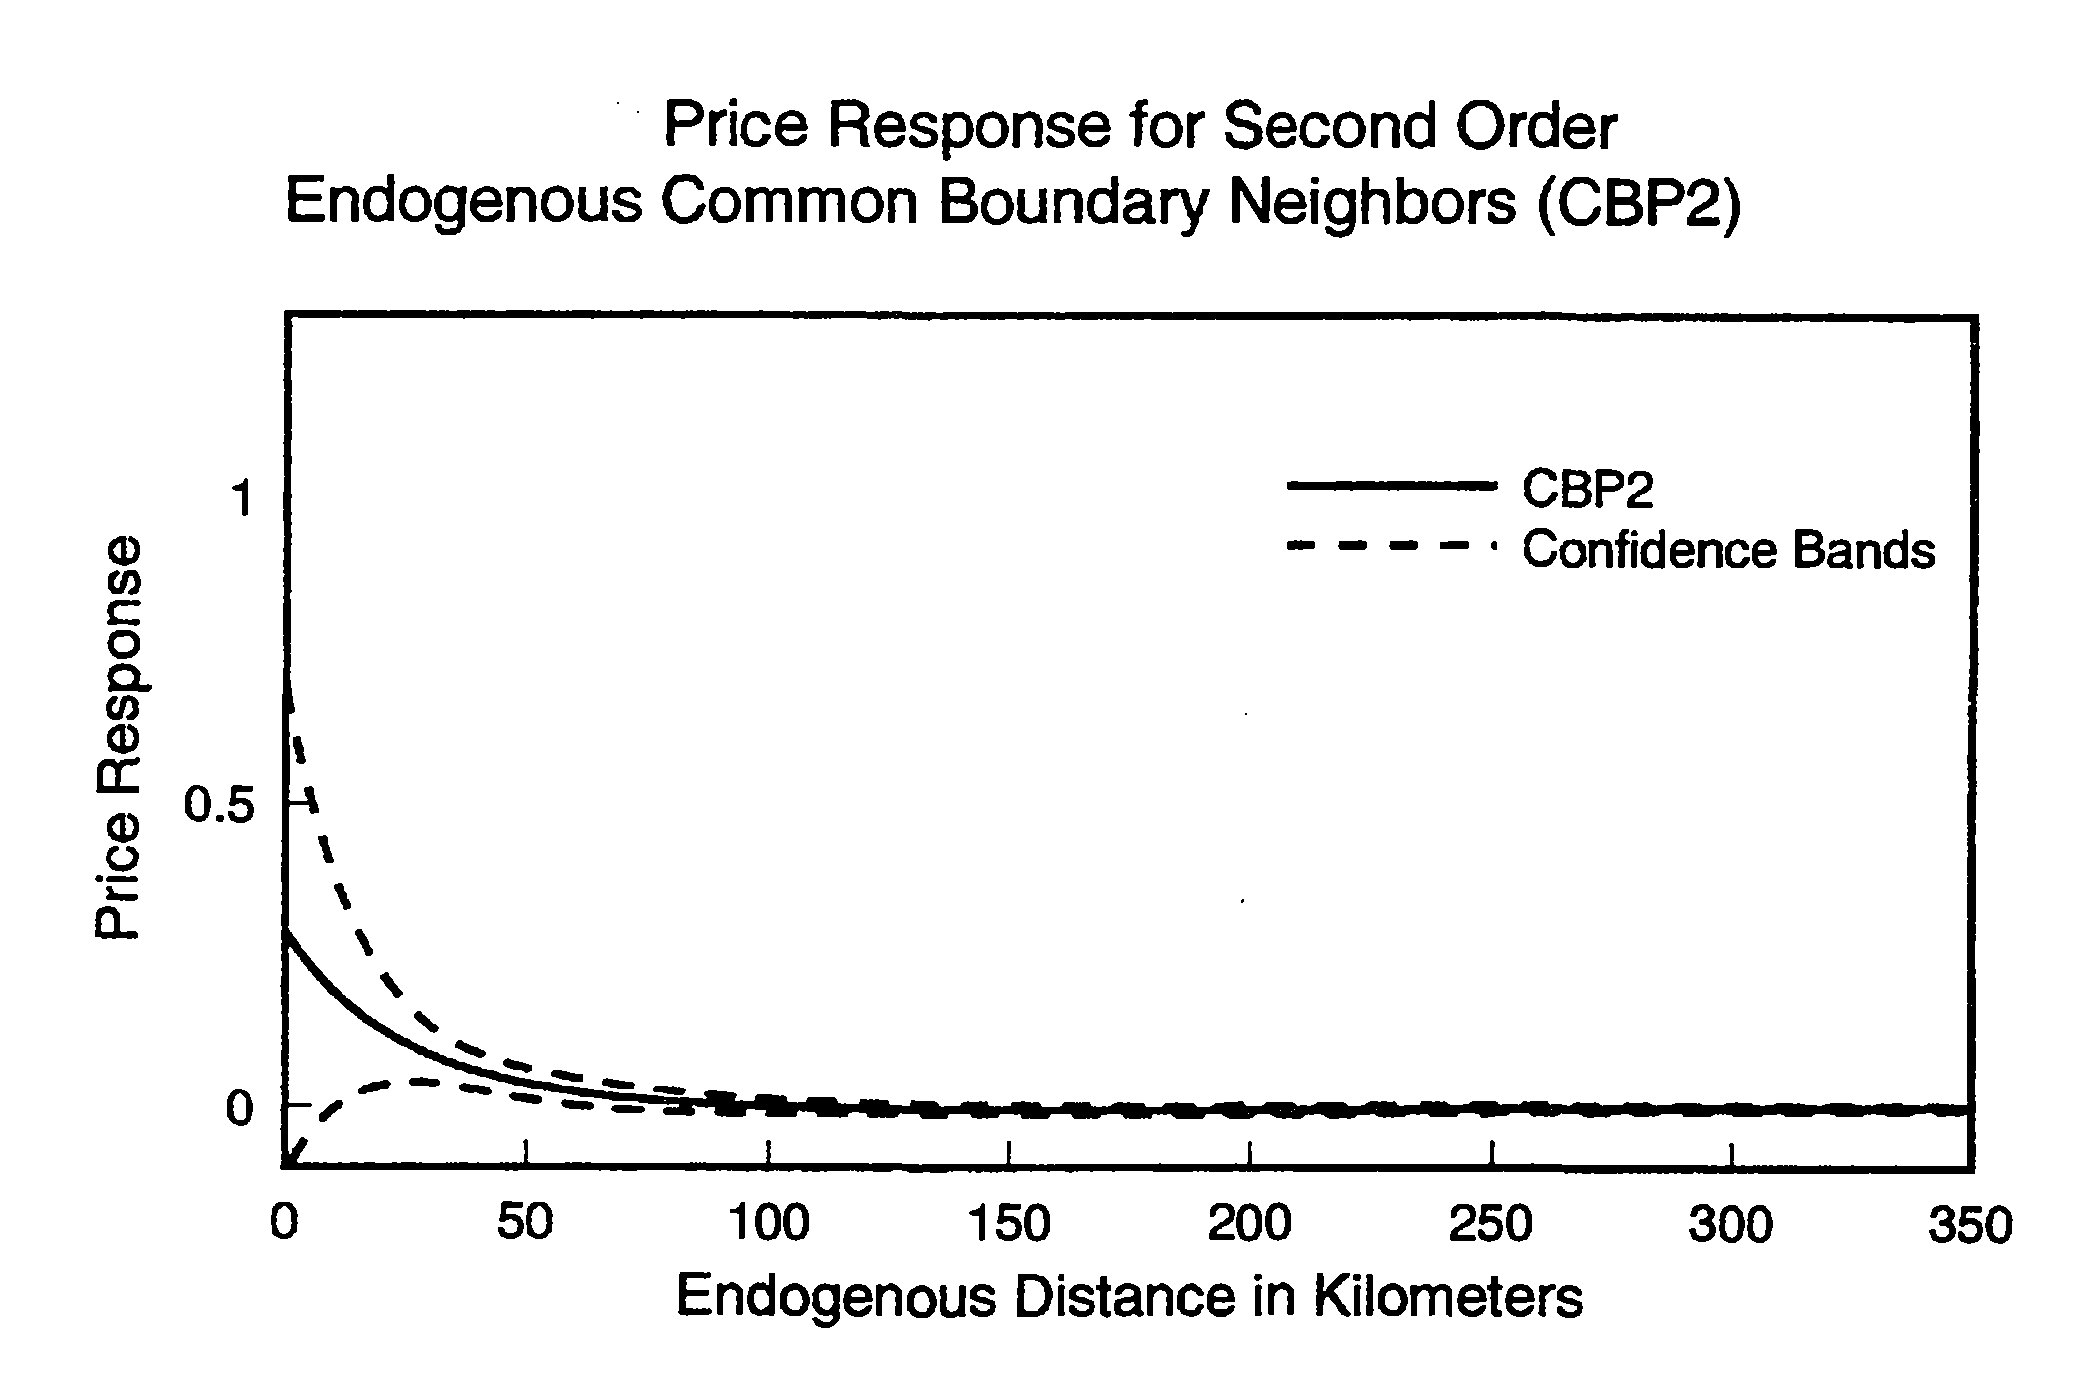
\includegraphics[width=\linewidth]{CBP2.png}
  \end{figure}
\end{frame}

\begin{frame}
  \frametitle{Semiparametric results}
  \vspace{-0.6cm}
  \begin{figure}
    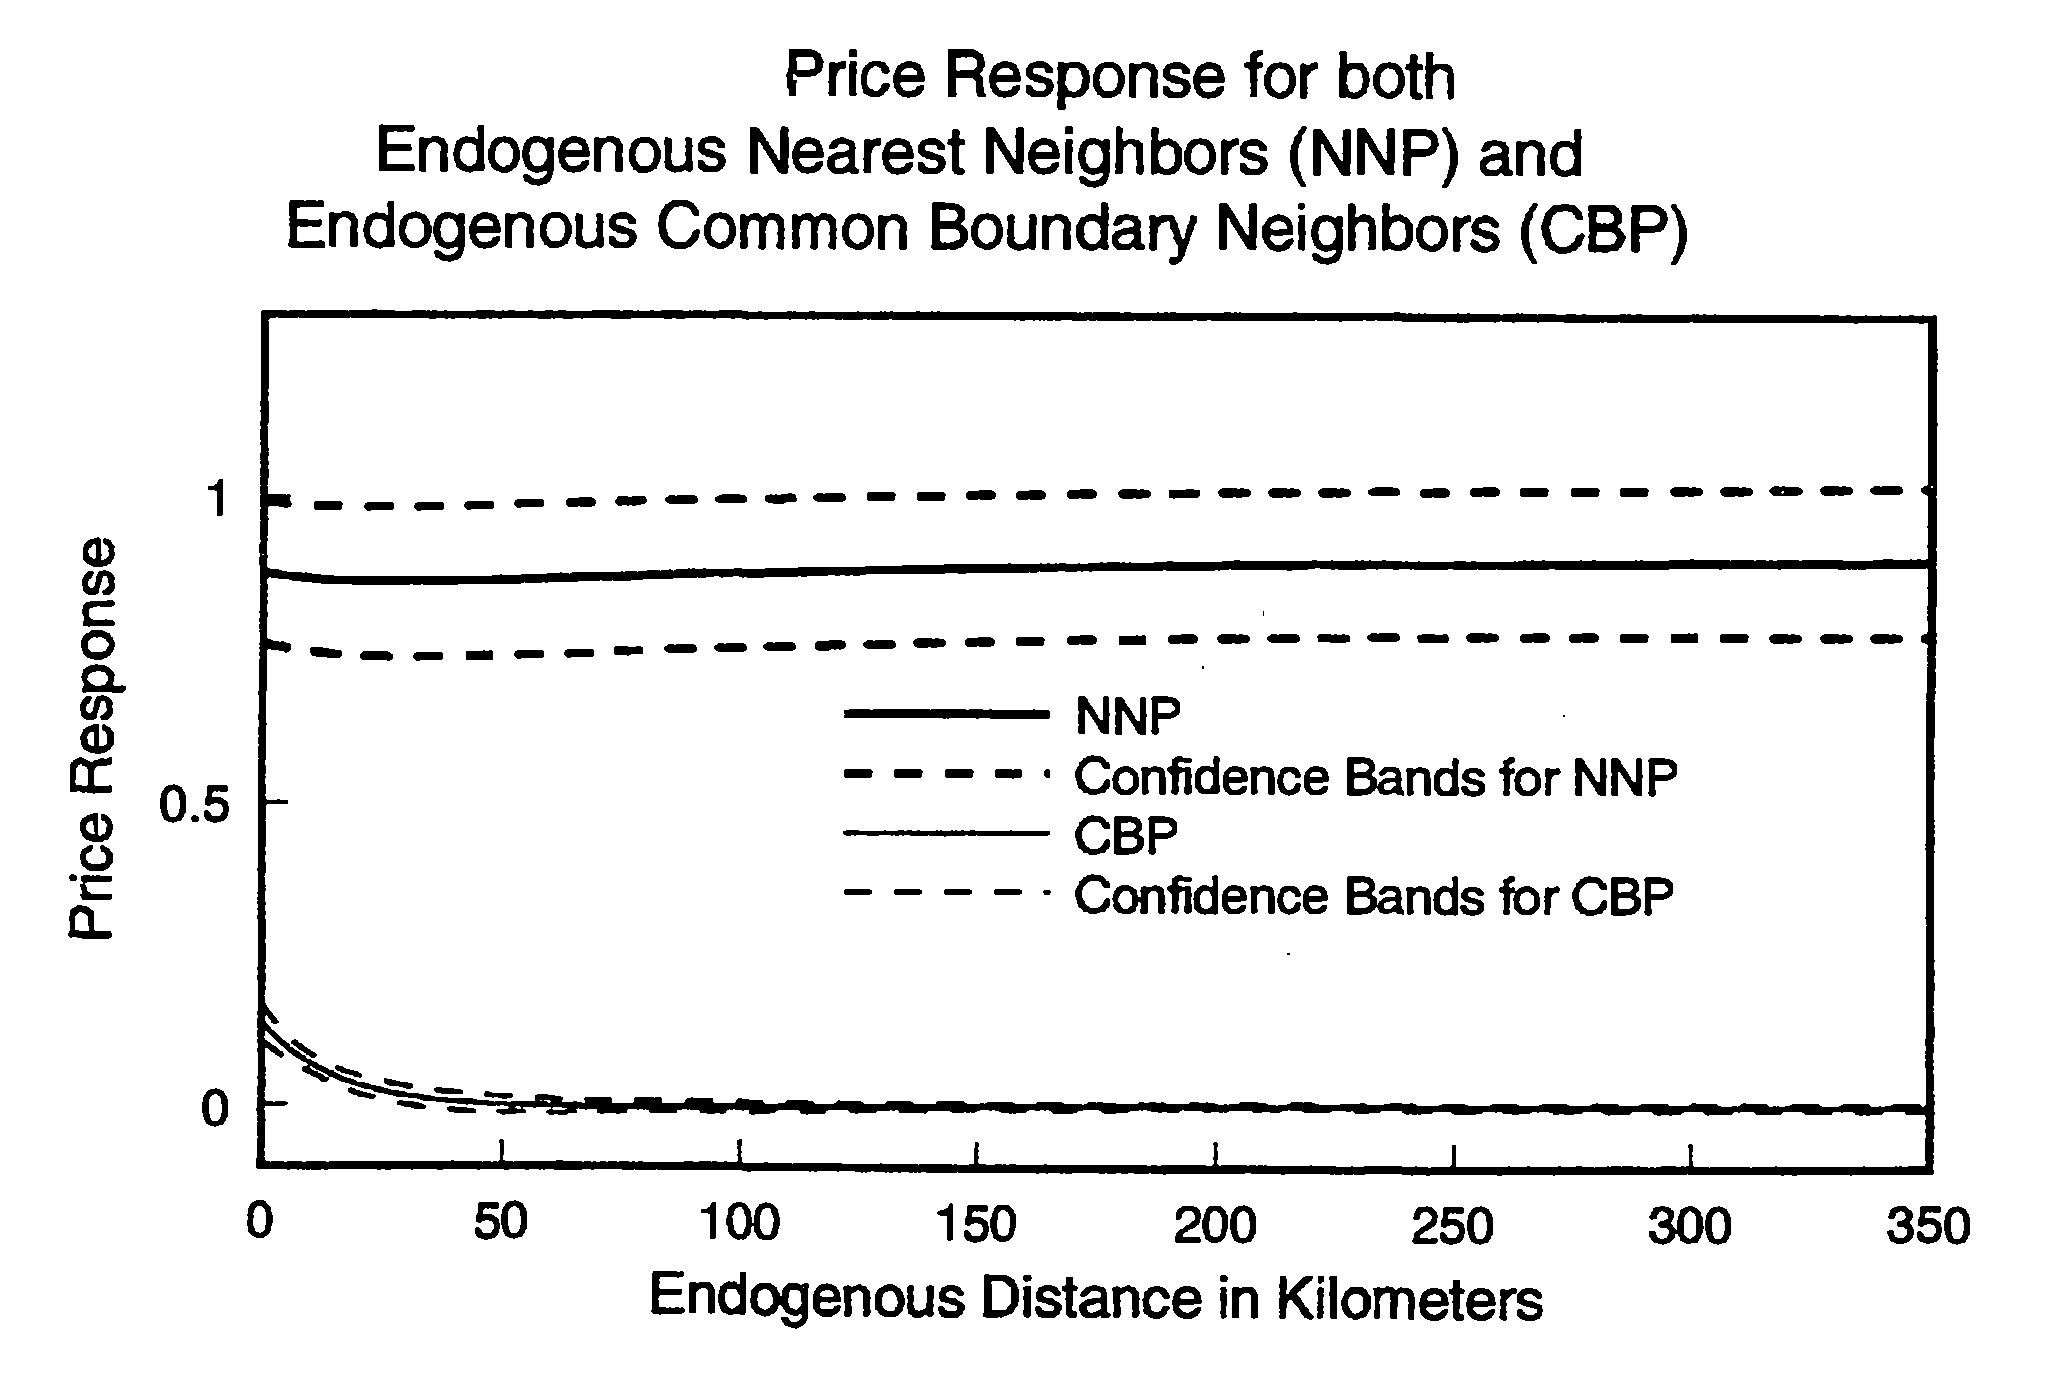
\includegraphics[width=\linewidth]{NNP&CBP.png}
  \end{figure}
\end{frame}

\begin{frame}
  \frametitle{Semiparametric results}
  \vspace{-0.6cm}
  \begin{figure}
    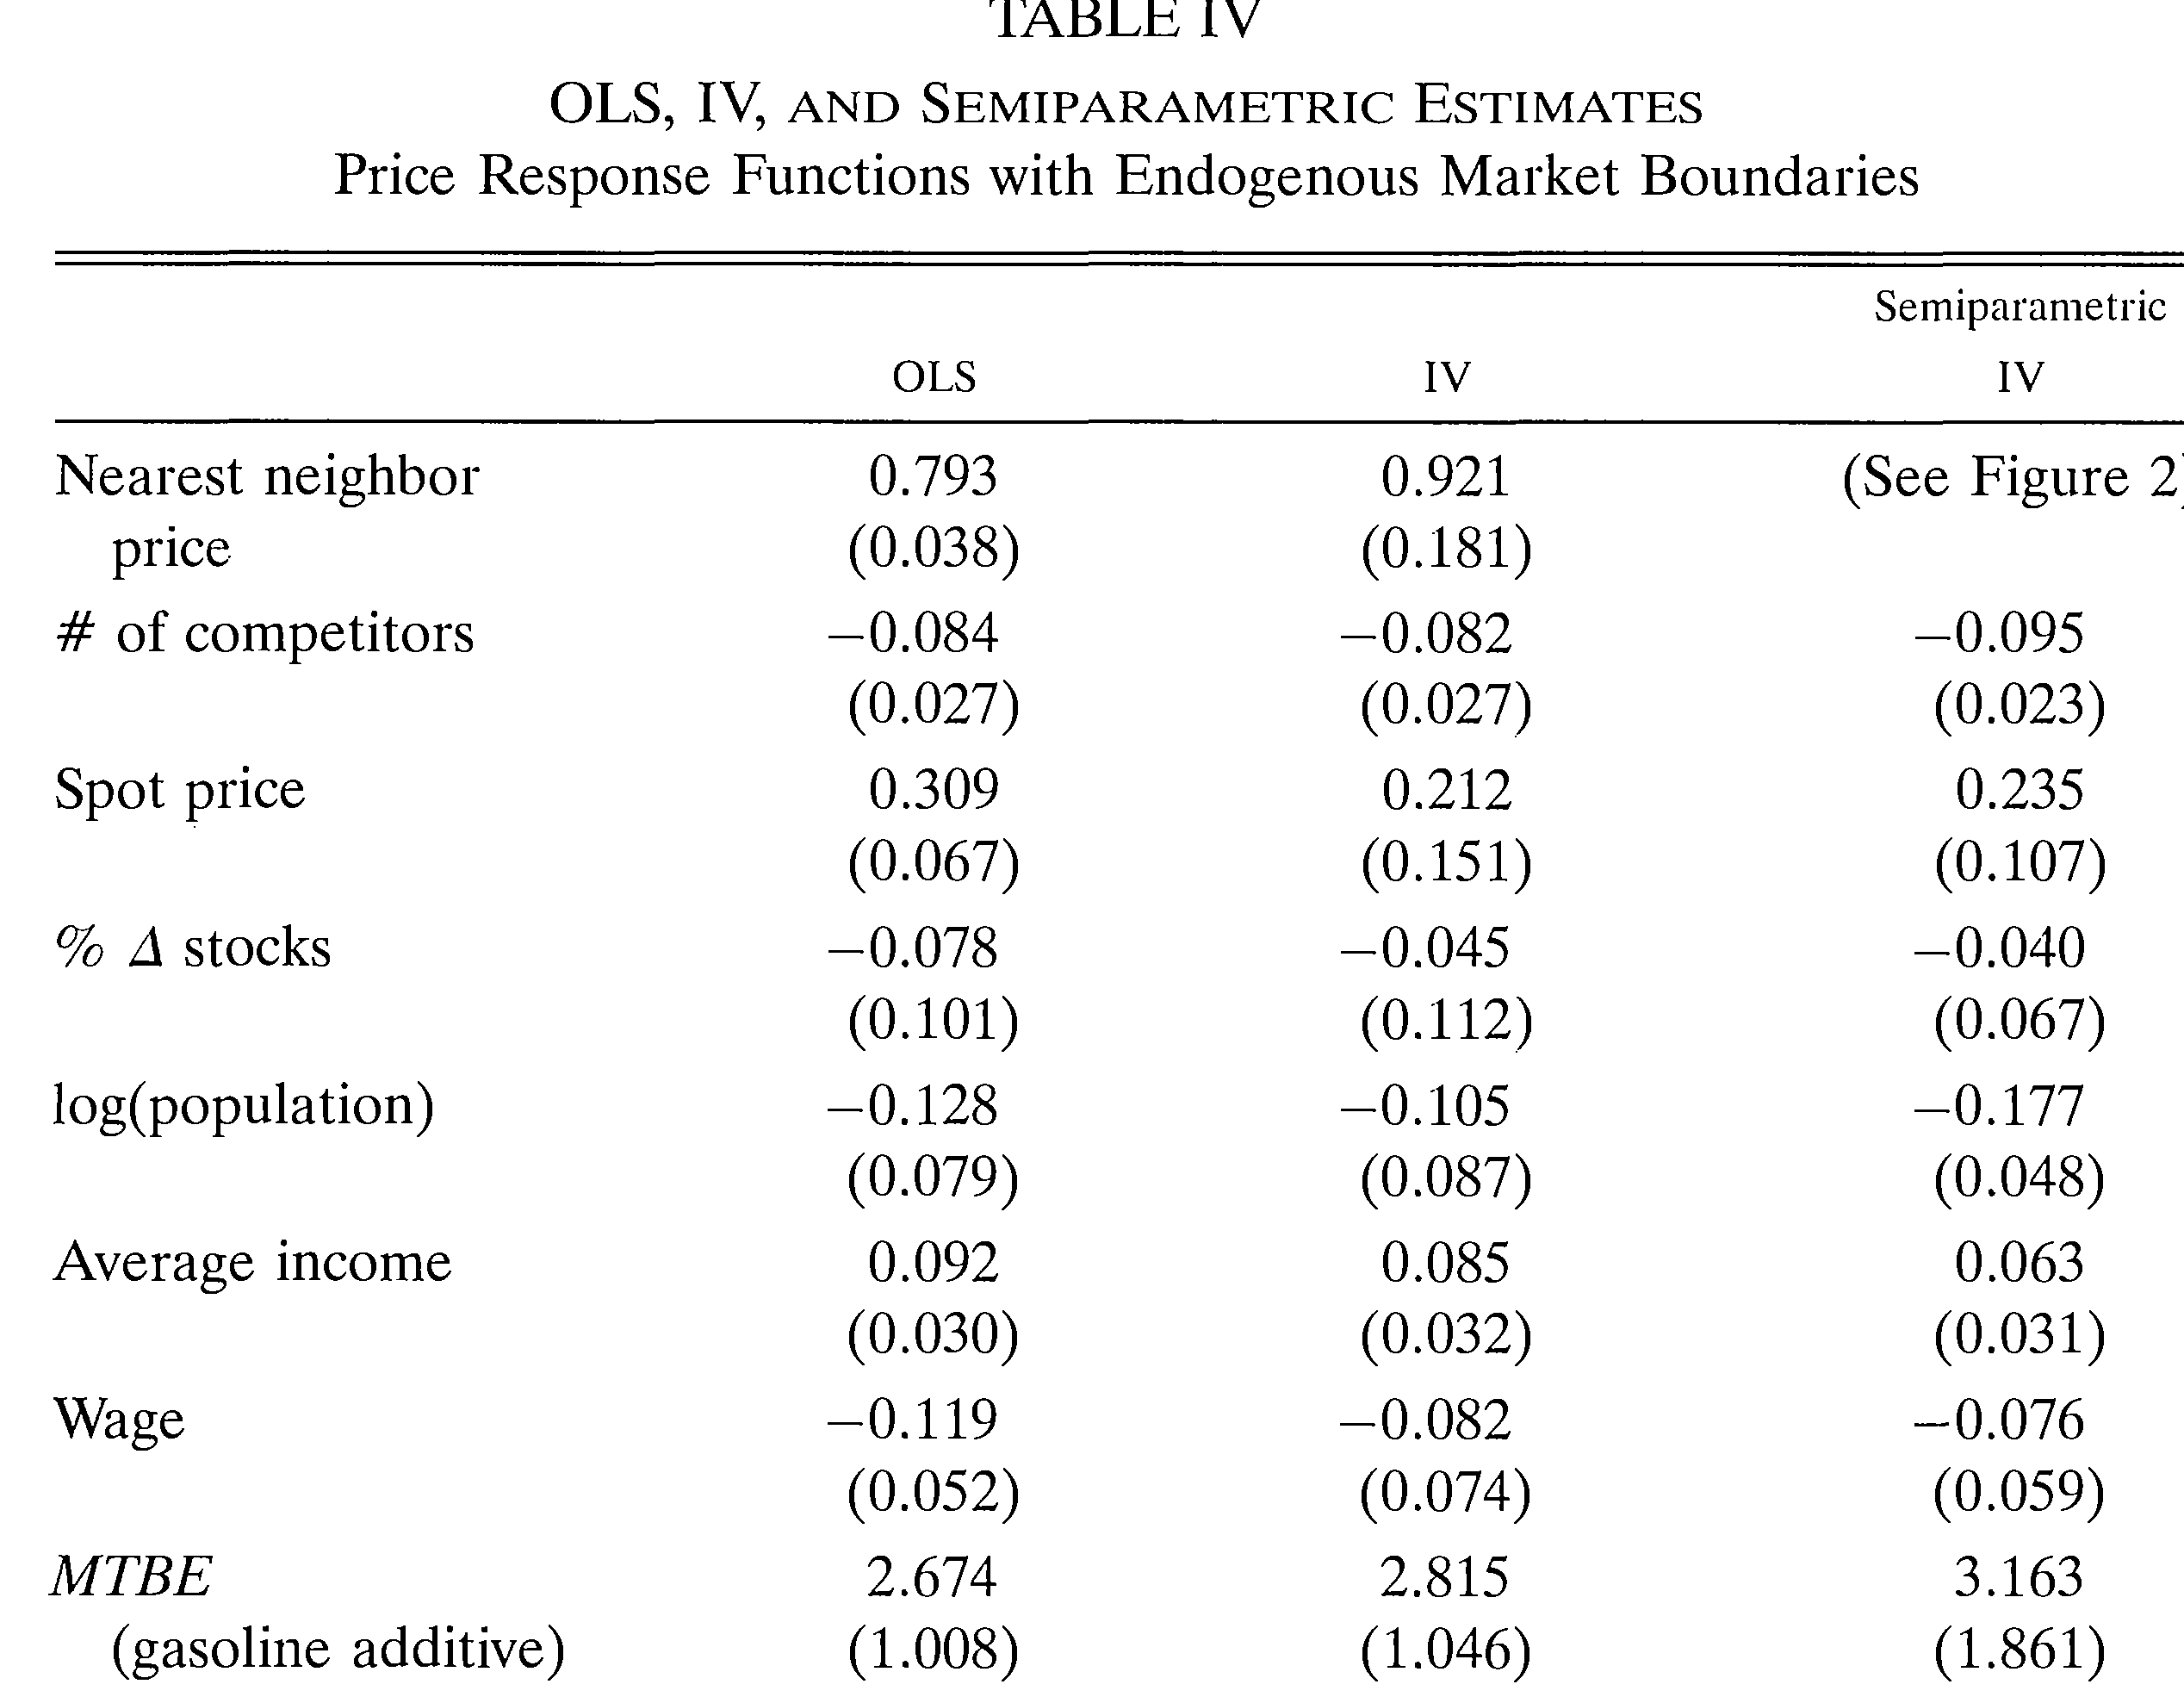
\includegraphics[width=\linewidth, height=7.5cm]{SemiPar_subres.png}
    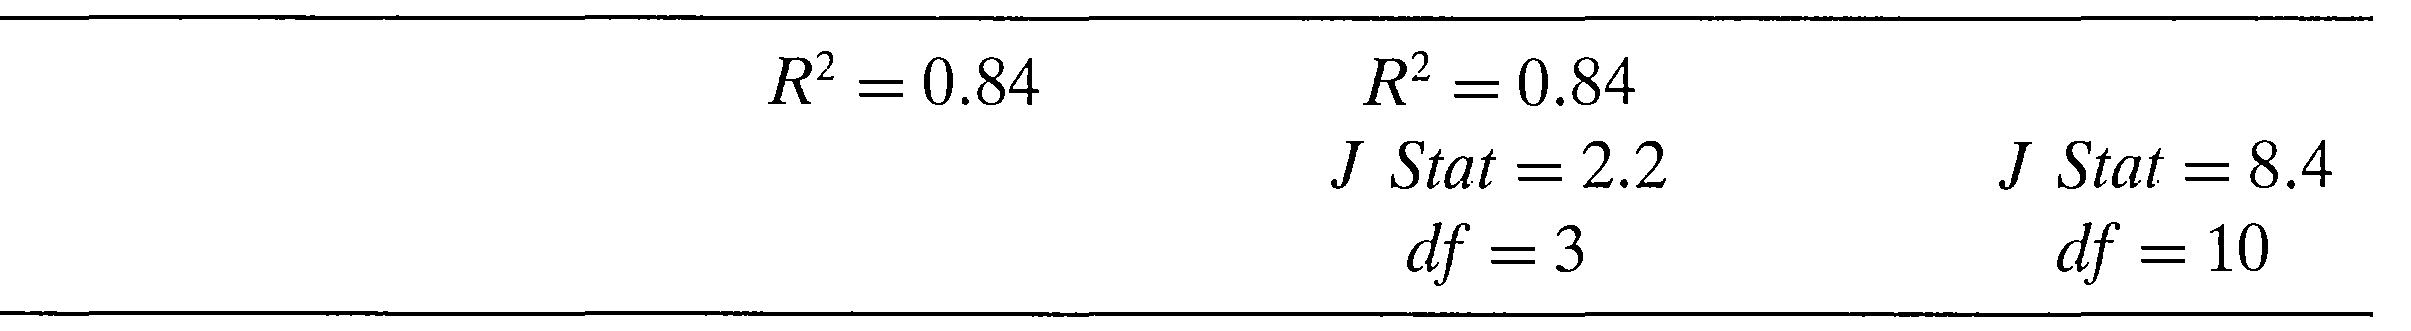
\includegraphics[width=\linewidth, height=1.2cm]{SemiPar_subres2.png}
  \end{figure}
\end{frame}

\begin{frame}
  \frametitle{Conclusion}
  \begin{itemize}
    \item The paper propose a method of estimating proximity that places minimal structure on the problem.
    \item Therefore multiple notion of distances can be tested and compared.
    \item Applying the method on the Wholesale Gasoline Market showed a market with highly localized competition.
    \item In fact, we seen that sellers compete only with the nearest terminal and ignore others even if it's a commomborder terminal.
    \item The same method could be applied in a number of other empirical research areas.
  \end{itemize}
  
\end{frame}

\end{document}

